\documentclass[UTF8]{ctexart}
\usepackage{geometry, CJKutf8}
\geometry{margin=1.5cm, vmargin={0pt,1cm}}
\setlength{\topmargin}{-1cm}
\setlength{\paperheight}{29.7cm}
\setlength{\textheight}{25.3cm}

% useful packages.
\usepackage{amsfonts}
\usepackage{amsmath}
\usepackage{amssymb}
\usepackage{amsthm}
\usepackage{enumerate}
\usepackage{graphicx}
\usepackage{multicol}
\usepackage{fancyhdr}
\usepackage{layout}
\usepackage{listings}
\usepackage{float, caption}
\usepackage{graphicx}
\usepackage{subcaption}
\lstset{
    basicstyle=\ttfamily, basewidth=0.5em
}

% some common command
\newcommand{\dif}{\mathrm{d}}
\newcommand{\avg}[1]{\left\langle #1 \right\rangle}
\newcommand{\difFrac}[2]{\frac{\dif #1}{\dif #2}}
\newcommand{\pdfFrac}[2]{\frac{\partial #1}{\partial #2}}
\newcommand{\OFL}{\mathrm{OFL}}
\newcommand{\UFL}{\mathrm{UFL}}
\newcommand{\fl}{\mathrm{fl}}
\newcommand{\op}{\odot}
\newcommand{\Eabs}{E_{\mathrm{abs}}}
\newcommand{\Erel}{E_{\mathrm{rel}}}

\begin{document}

\pagestyle{fancy}
\fancyhead{}
\lhead{韩箫, 32301000653}
\chead{数据结构与算法项目作业}
\rhead{\today}

\setlength{\parindent}{2em}

\section{\texttt{expression\_evaluator.h}的设计思路}

我自定义了一个类arithmetic,用于接收外界输入的字符串,完成表达式的中缀、后缀转化,错误检验,表达式计算求值,以及最后输出的功能。

先阐释分析类的private部分成员。
\subsection{成员变量}
\begin{enumerate}
\item stack<char> operators存放运算符,用于中缀转后缀时的运算符优先级比较与输出。
\item string postfix\_expression存放转换后的后缀表达式。
\item stack<double> numbers存放操作数,用于后缀表达式的计算求值。
\item indicator用于标记表达式是否合法,若合法则为true,否则为false。如果表达式不合法,将直接返回,停止该表达式的计算,进入测试程序中下一个表达式的计算。
\end{enumerate}
\subsection{\texttt{priority}函数}
预备函数,用于定义运算符的优先级,在中后缀转化时可以直接调用。同时兼具判断未定义字符的功能。
\subsection{\texttt{right\_bracket}函数}
预备函数,用于集中处理右括号的情况。因为右括号处理的逻辑都是一致的,都是不断弹出运算符,连接到后缀表达式,直到遇见对应左括号为止(左括号不入序列),故可集成处理。
同时,兼具判断括号是否匹配的功能,若运算符全部输出,仍未遇到匹配的左括号则表达式不合法。
\subsection{\texttt{transform}函数}
本函数是整个类的\textbf{核心函数}之一,用于将中缀表达式转化为后缀表达式。
因为需要判断表达式的合法性,采用比较朴实的方法,定义了四个指示变量,用于记录表达式的不同部分和运算阶段。
\begin{enumerate}
\item \texttt{flag}用于指示运算符的连续出现个数。为了应对开头是运算符的情况,将初值设为1。正常情况下(负号另行考虑),flag为0-1变量,若flag为2则运算符连续出现,表达式不合法。
\item \texttt{digit}用于小数点前位数计数,检验是否符合科学计数法规范,与下一个\texttt{point}变量配合使用。
\item \texttt{point}用于标记是否进入小数部分,检验是否符合科学计数法规范。
\item \texttt{notion}用于标记是否进入科学计数法的幂次部分。
\end{enumerate}

接下来,根据输入的中缀表达式逐个字符处理,根据字符的不同情况分类讨论。
\subsubsection{数字情形}
数字,小数点,以及科学计数法e实际都为数字部分,整体考虑,除了非法判断分别处理。都直接加入后缀表达式中,同时将flag置零,因为只有数字能打断运算符的连续出现。
各指示变量按照实际情况进行维护。

如果科学计数法的e前的整数位数超过一位,或幂次不为整数,则表达式不合法。都通过notion、point、digit变量配合判断。
\subsubsection{运算符'+''-''*'情形}
根据优先级统一处理,维护各指示变量。运算符及括号标志数字结束,如果前面的数字为科学计数法,在末尾加'E'作为标记,便于后续计算。若运算符连续出现,直接退出报错。同时为了分隔各操作数,在运算符前加入空格,便于后续计算。
\subsubsection{'-'情形}
负号的处理比较特殊,可能是负号或减号,通过flag变量的值进行区分。

若flag为1,根据我的程序定义逻辑为负号,直接加入后缀表达式中。若flag为0,则为减号,按运算符处理。

若flag大于1,说明运算符连续出现,不合法,直接退出报错。
\subsubsection{括号情形}
左括号推入栈中,维护各指示变量。右括号调用\texttt{right\_bracket}函数处理。
\subsubsection{未定义字符情形}
直接退出报错。

\subsection{\texttt{calculate}函数}
本函数是整个类的另一个\textbf{核心函数},用于计算后缀表达式的值。表达式本身的格式合法与否已由\texttt{transform}函数完成判断,本函数无需考虑。

根据后缀表达式的特点,从左到右逐个扫描,遇到数字直接入栈,遇到运算符弹出两个数字进行运算,结果入栈。
0-1指示变量flag用于表示数字即将开始。根据\texttt{transform}函数的定义,后缀表达式中的空格只出现在数字(包括负数)之前。为保持逻辑一致,初值设为1。
如果遇到空格或e,flag置1,表示数字即将开始。
\subsubsection{数字情形}
Line 214-229的if-else语句,整体用于处理数字(包括负数)的情况,并转化为浮点数。
直接将负号、数字、小数点加入字符串num中,遇到其它符号时,表示数字部分结束,将字符串转化为浮点数,入栈。

\textbf{注意}:负号情况下,flag不可置零!必须出现数字才能置零。因为该组判断与下一组if-else的运算判断独立,置零后会满足下一组if-else条件,引发段错误!
\subsubsection{运算符情形}
Line 231-250的if-else语句,整体用于处理运算符的情况。

此处将\texttt{transform}中加入的指示符'E'也当作运算符处理,用于计算科学计数法的结果(因为事实上,也是e前后两个操作数完成的计算)。
数字栈中弹出两个操作数,基本运算直接调用\texttt{fundamental}函数,同时对除数为零的情况进行判断和报错。

\subsection{两个打印函数}
\texttt{print}用于打印后缀表达式,主要用于编程过程中检查中间步骤的正确性。 

\texttt{print\_result}函数打印计算结果,如果indicator指示报错则不打印。
\clearpage
public部分:
\subsection{\texttt{calculation}函数}
集成了接收外界输入,调用私有函数完成计算,输出结果的功能。
同时在各步骤过程中都及时判断是否出错,若出错则暂停该表达式求值,进入测试程序下一个表达式。

\section{测试函数}
测试了以下几种类型的表达式,详见\texttt{test.cpp}文件。
\begin{enumerate}
    \item 基本的加、减、乘、除运算以及括号的处理。
    \item 检验中括号的处理。
    \item 检验大括号。
    \item 括号不配对的情况。
    \item 更多括号不配对。
    \item 检验除数为零的情况。
    \item 表达式中包含未定义字符的情况。
    \item 检验运算符连续出现。
    \item 检验运算符在表达式开头的情况。
    \item 表达式中间包含负数的情况。
    \item 开头包含负数的情况。
    \item 开头包含科学计数法。
    \item 科学计数法,幂次为负数。
    \item 检验科学计数法不合规范的情况。
    \item 包含小数的运算。
    \item 检验科学计数法幂次非法的情况。
\end{enumerate}
\clearpage
\section{运行结果}
如下图所示,测试程序运行结果正确,所有测试用例均符合理论预期。
\begin{figure}[H]
    \centering
    \begin{subfigure}[b]{0.5\textwidth}
        \centering
        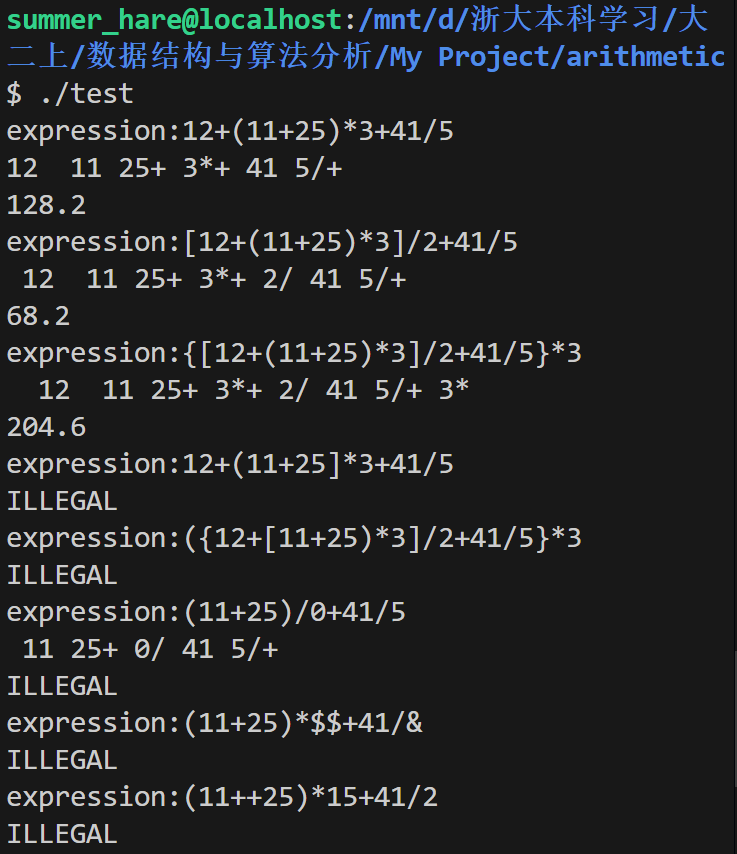
\includegraphics[width=\textwidth]{result1.png}
        \caption{a}
        \label{fig:result1}
    \end{subfigure}
    \hfill
    \begin{subfigure}[b]{0.4\textwidth}
        \centering
        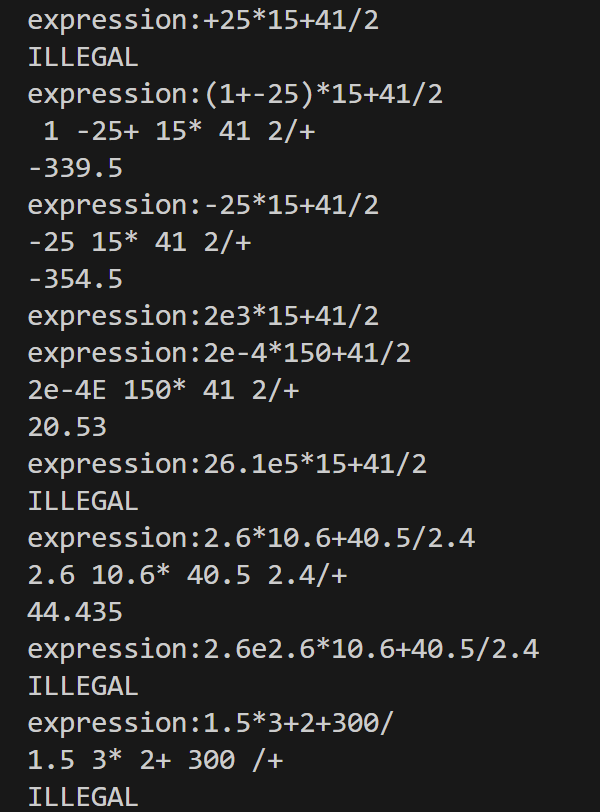
\includegraphics[width=\textwidth]{result2.png}
        \caption{b}
        \label{fig:result2}
    \end{subfigure}
    \caption{测试程序运行结果}
    \label{fig:results}
\end{figure}




\section*{完结撒花!}

\end{document}

%%% Local Variables: 
%%% mode: latex
%%% TeX-master: t
%%% End: 
